\documentclass[tikz, border=5mm]{standalone}

\usetikzlibrary{arrows.meta,decorations.markings,fit,calc, positioning}

\definecolor{componentColor}{RGB}{210,210,210}
\definecolor{systemColor}{RGB}{230,230,230}

\tikzset{component/.append style={fill=componentColor, align=center, draw, minimum width=2cm, minimum height=1.5cm, rounded corners=.3cm}}
\tikzset{system/.style={component, fill=systemColor, rounded corners=0cm}}
\tikzset{interface/.style={system, fill=systemColor, minimum size=1.6cm}}

\tikzstyle{arrow} = [-{Latex[scale=3.0]}]
\tikzset{arrowLabel/.append style={minimum height=.25cm, draw=none}}
\begin{document}

	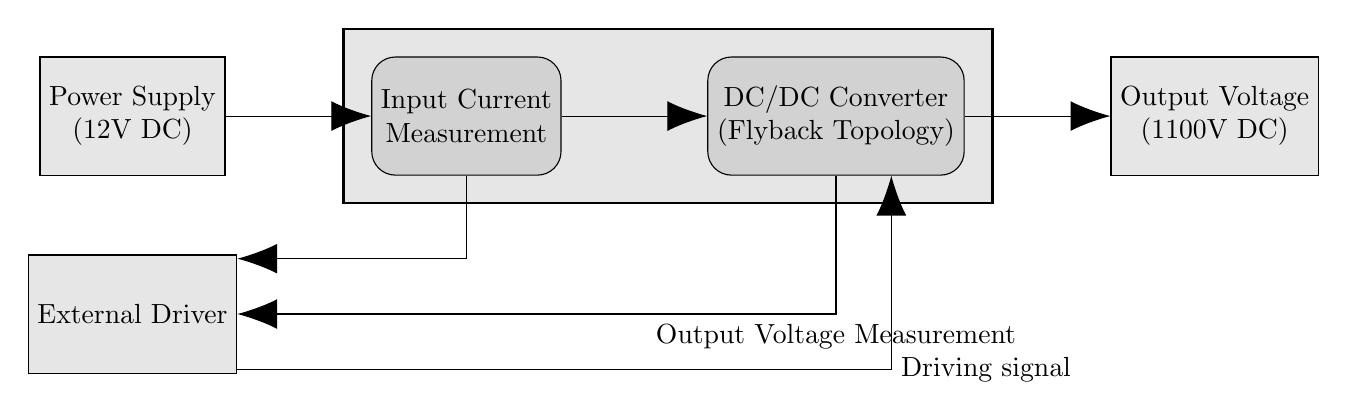
\begin{tikzpicture}[node distance=1.0cm and 1.85cm]
	% Nodes
	\pgfdeclarelayer{background}
	\pgfsetlayers{background,main}
	
		\node (vcc) [system] {Power Supply\\ (12V DC)};

		\node (currentlevel) [component, right=of vcc] {Input Current\\ Measurement};
        \node (converter) [component, right=of currentlevel] {DC/DC Converter\\ (Flyback Topology)};	
        
		\node (vout) [system, right=of converter] {Output Voltage\\ (1100V DC)};       
        \node (driver) [system, below=of vcc] {External Driver};

		\begin{pgfonlayer}{background}
		\node[system, draw, thick, inner xsep=1em, inner ysep=1em, fit= (currentlevel) (converter)] {};
		\end{pgfonlayer}

		% Connectors
		\begin{scope}[->]
		
            \draw [arrow] (vcc) -- (currentlevel);
            \draw [arrow] (currentlevel) -- (converter);
            \draw [arrow] (converter) -- (vout);	
			\draw [arrow] (currentlevel.south) -| ++(0,0) |- ([yshift=20]driver.east);
			\draw [arrow] (converter.south) -| ++(0,0)  |- node[anchor=north, minimum width=.25cm, draw=none]{{Output Voltage Measurement}}  (driver.east);
			\draw [arrow] ([yshift=-20]driver.east) |- ++(0,0) -| node[anchor=west, minimum width=.25cm, draw=none]{{Driving signal}} ([xshift=20]converter.south);
	    \end{scope}
\end{tikzpicture}
\end{document}
